\begin{greek}
\chapter{Συλλογή σκουπιδιών με σήμανση και εκκαθάριση}\label{ch:mrkswp}

Ο ιδανικός στόχος ενός συλλέκτη σκουπιδιών είναι η ανάκτηση
του χώρου που καταλαμβάνει κάθε αντικείμενο το οποίο δεν
πρόκειται να ξαναχρησιμοποιηθεί από το πρόγραμμα. Κάθε
σύστημα αυτόματης διαχείρισης μνήμης είναι επιφορτισμένο με
τις εξής υποχρεώσεις:

\begin{enumerate}
  \item να εκχωρεί χώρο για νέα αντικείμενα,
  \item να αναγνωρίζει τα ζωντανά αντικείμενα,
  \item να ανακτά το χώρο που καταλαμβάνουν τα νεκρά αντικείμενα.
\end{enumerate}

Οι υποχρεώσεις αυτές δεν είναι ανεξάρτητες. Πιο συγκεκριμένα,
ο τρόπος ανάκτησης μνήμης επηρεάζει την εκχώρηση μνήμης. Όπως
είδαμε στο κεφάλαιο~\ref{ch:intro}, το πρόβλημα της απόφασης
κατά πόσο ένα αντικείμενο είναι πραγματικά ζωντανό είναι
μη-αποφασίσιμο. Η προσβασιμότητα μέσω δεικτών δίνει μία
υπερ-προσέγγιση του συνόλου των ζωντανών αντικειμένων. Ένα
αντικείμενο θεωρείται ζωντανό αν και μόνο αν είναι προσβάσιμο
δια μέσου μιας αλυσίδας αναφορών ξεκινώντας από ένα σύνολο
(γνωστών) ριζών. Από την άλλη πλευρά, ένα αντικείμενο θεωρείται
νεκρό και η μνήμη που αυτό καταλαμβάνει μπορεί να ανακτηθεί,
αν δεν είναι προσβάσιμο από καμία τέτοια αλυσίδα αναφορών.
Παρότι ένα ζωντανό αντικείμενο ενδέχεται να μην προσπελασθεί
ξανά, ένα νεκρό αντικείμενο είναι σίγουρα νεκρό.

\begin{algorithm}
  \caption{Σήμανση-εκκαθάριση: εκχώρηση}
  \label{alg:mrkswp_1}
  \begin{algorithmic}[1]
    \Procedure{New}{\null}
      \State $ref \gets$ \Call{allocate}{\null}
      \If{$ref = \textbf{null}$} \Comment{heap is full}
        \State \Call{collect}{\null}
        \State $ref \gets$ \Call{allocate}{\null}
        \If{$ref = \textbf{null}$}
          \Comment{heap is still full}
          \State error ``Out of memory!''
        \EndIf
      \EndIf
      \State \Return{$ref$}
    \EndProcedure
    \Statex
    \Procedure{collect}{\null}
      \State \textbf{atomic}
      \State \Call{markFromRoots}{\null}
      \State \Call{sweep}{$start$, $end$}
    \EndProcedure
  \end{algorithmic}
\end{algorithm}

Ο πρώτος αλγόριθμος που εξετάζουμε είναι αυτός της 
\textbf{συλλογής με σήμανση και εκκαθάριση} και διατυπώθηκε από
τον Collins \cite{DBLP:journals/cacm/McCarthy60}. Πρόκειται για
μια απευθείας υλοποίηση της αναδρομικής ιδιότητας της προσβασιμότητας
μέσω δεικτών. Ο αλγόριθμος εκτελείται σε δύο φάσεις: αρχικά ο
συλλέκτης διασχίζει το γράφο των αντικειμένων, εκκινώντας από
τις ρίζες (καταχωρητές, στοίβα, καθολικές μεταβλητές), δια μέσου
των οποίων το πρόγραμμα έχει άμεση πρόσβαση σε αντικείμενα
και συνεχίζει ακολουθώντας μεταβλητές δείκτες και σημαίνοντας
κάθε αντικείμενο που συναντά. Η πρώτη αυτή φάση είναι γνωστή και
ως \textbf{εξιχνίαση}. Στη δεύτερη φάση, αυτήν της \textbf{εκκαθάρισης},
ο συλλέκτης εξετάζει κάθε αντικείμενο στο σωρό: κάθε μη-σημασμένο
αντικείμενο θεωρείται σκουπίδι και η μνήμη που αυτό καταλαμβάνει
απελευθερώνεται.

Ακριβώς επειδή δεν εντοπίζει τα σκουπίδια καθεαυτά, αλλά αντίθετα 
εντοπίζει τα αντικείμενα που δεν είναι σκουπίδια και έπειτα 
συμπεραίνει πώς τα υπόλοιπα είναι σκουπίδια, ο αλγόριθμος με 
σήμανση και εκκαθάριση χαρακτηρίζεται πολλές φορές και ως
\textbf{έμμεσος}. Κάθε φορά που εκτελείται, εντοπίζει 
από την αρχή τα προσβάσιμα αντικείμενα. Αντίθετα, ένας 
\textbf{άμεσος} αλγόριθμος συλλογής αποφαίνεται κατά 
πόσο ένα αντικείμενα είναι ενεργό ή μή από το αντικείμενο καθεαυτό, 
χωρίς να είναι απαραίτητη η διάσχιση του γράφου των αντικειμένων. 
Παράδειγμα ενός άμεσου αλγορίθμου αποτελεί ο αλγόριθμος 
καταμέτρησης αναφορών.

\section{Ο αλγόριθμος}
Από την πλευρά του συλλέκτη, τα νήματα τροποποιητές εκτελούν 3 
ενδιαφέρουσες ενέργειες τις \textproc{New}, \textproc{Read} και
\textproc{Write}, τις οποίες κάθε αλγόριθμος συλλογής ορίζει
με το δικό του τρόπο. Η διαπροσωπεία του συλλέκτη με τον τροποποιητή
είναι ιδιαίτερα απλή. Αν δεν είναι δυνατή η εκχώρηση μνήμης για 
ένα αντικειμένο σε ένα νήμα, καλείται ο συλλέκτης και το αίτημα 
εκχώρησης επαναλαμβάνεται. Η παρουσία της λέξης κλειδί 
\textbf{atomic} τονίζει πώς η εκτέλεση του συλλέκτη πραγματοποιείται
με παύση του κόσμου, δηλαδή χωρίς να εκτελούνται ταυτόχρονα νήματα
τροποποιητές. Αν και πάλι το αίτημα δεν μπορεί ικανοποιηθεί, η
διαθέσιμη μνήμη στο σωρό έχει εξαντληθεί. Ενώ τις περισσότερες 
φορές αυτό αποτελεί σφάλμα εκτέλεσης, σε ορισμένες γλώσσες
προγραμματισμού η συνάρτηση \textproc{New} δύναται να εγείρει
μία εξαίρεση την οποία ο προγραμματιστής μπορεί να πιάσει και
να χειριστεί.

\begin{algorithm}
  \caption{Σήμανση-εκκαθάριση: σήμανση}
  \label{alg:mrkswp_2}
  \begin{algorithmic}[1]
    \Procedure{markFromRoots}{\null}
      \State \Call{initialize}{$worklist$}
      \ForAll{$fld \in Roots$}
        \State $ref \gets *fld$
        \If{$ref \neq \textbf{null}$ \textbf{and} \textbf{not} \Call{isMarked}{$ref$}}
          \State \Call{setMarked}{$ref$}
          \State \Call{add}{$worklist$, $ref$}
          \State \Call{mark}{\null}
        \EndIf
      \EndFor
    \EndProcedure
    \Statex
    \Procedure{initialize}{\null}
      \State $worklist \gets empty$
    \EndProcedure
    \Statex
    \Procedure{mark}{\null}
      \While{\textbf{not} \Call{isEmpty}{$worklist$}}
        \State $ref \gets$ \Call{remove}{$worklist$}
        \ForAll{$fld \in Pointers(ref)$}
          \State $child \gets *fld$
          \If{$child \neq \textbf{null}$ \textbf{and} \textbf{not} \Call{isMarked}{$child$}}
            \State \Call{setMarked}{$child$}
            \State \Call{add}{$worklist$, $child$}
          \EndIf
        \EndFor
      \EndWhile
    \EndProcedure
  \end{algorithmic}
\end{algorithm}

Πριν ξεκινήσει την εξερεύνηση του γράφου αντικειμένων, ο
συλλέκτης πρέπει να αρχικοποιήσει τη λίστα εργασιών ($worklist$) 
με τα αντικείμενα εκκίνησης της εξερεύνησης (διαδικασία
\textproc{markFromRoots}). Κάθε αντικείμενο ρίζα σημαίνεται 
και τοποθετείται στη λίστα εργασιών. Η σήμανση κωδικοποιείται 
συνήθως με την τιμή ενός bit/byte το οποίο αποθηκεύεται είτε 
στην κεφαλίδα του αντικειμένου είτε σε έναν ξεχωριστό πίνακα 
(bitmap table). Αν ένα αντικείμενο δεν περιέχει δείκτες, 
απλώς σημαίνεται και δεν εισάγεται στη λίστα εργασιών, αφού 
αυτό δεν είναι απαραίτητο καθώς δεν έχει παιδιά. Για να
ελαχιστοποιηθεί το μέγεθος της λίστας εργασιών, η 
\textproc{markFromRoots} καλεί αμέσως τη διαδικασία
\textproc{mark}. Εναλλακτικά, μπορεί να είναι επιθυμητή
η όσο το δυνατόν γρηγορότερη σάρωση των ριζών κάθε νήματος
τροποποιητή. Για παράδειγμα ένας ταυτόχρονος συλλέκτης 
μπορεί να διακόπτει την εκτέλεση ενός νήματος για πολύ
μικρό χρονικό διάστημα ώστε να σαρώσει τη στοίβα του
και να συνεχίσει με την εξερεύνηση του γράφου ενώ το
τελευταίο εκτελείται.

Η λίστα εργασιών μπορεί να υλοποιηθεί ως μία στοίβα, οδηγώντας 
έτσι σε μία κατά βάθος διάσχιση του γράφου των αντικειμένων. 
Αν μάλιστα τα bit σήμανσης βρίσκονται αποθηκευμένα μαζί με 
τα αντικείμενα (π.χ στην κεφαλίδα των τελευταίων), τότε τα 
επόμενα αντικείμενα που πρόκειται να εξεταστούν, αυτά που 
είναι ήδη σημασμένα, βρίσκονται με μεγάλη πιθανότητα στην 
μνήμη cache. Η τοπικότητα των αναφορών μπορεί να επιδράσει
σε μεγάλο βαθμό την επίδοση του συλλέκτη.

Η σήμανση του γράφου των αντικειμένων υλοποιείται από έναν 
απλό βρόχο while. Ο δείκτης σε ένα αντικείμενο εξάγεται από 
τη λίστα εργασιών και οι δείκτες του αντικειμένου αυτού, 
εφόσον δε δείχνουν σε σημασμένα αντικείμενα εισάγονται σε 
αυτή, μέχρις ότου η λίστα εργασιών αδειάσει. Σε αυτήν την
εκδοχή της \textproc{mark} κάθε αντικείμενο προς το οποίο
υπάρχει αναφορά στη λίστα εργασιών είναι σημασμένο. 
Ο τερματισμός της διαδικασίας \textproc{mark}, επομένως και 
της \textproc{markFromRoots} εξασφαλίζεται από το γεγονός 
πώς ένας δείκτης σε ήδη σημασμένο αντικείμενο δεν εισάγεται 
στη λίστα εργασιών. Κατά την επιστροφή της \end{greek} \textproc{markFromRoots}, \begin{greek} 
κάθε αντικείμενο που είναι προσβάσιμο από τις ρίζες του 
προγράμματος έχει σημανθεί. Κάθε μη σημασμένο αντικείμενο 
είναι σκουπίδι και η μνήμη που αυτό καταλαμβάνει μπορεί να 
απελευθερωθεί.

\begin{algorithm}
  \caption{Σήμανση-εκκαθάριση: εκκαθάριση}
  \label{alg:mrkswp_3}
  \begin{algorithmic}[1]
    \Procedure{sweep}{$start$, $end$}
      \State $scan \gets start$
      \While{$scan < end$}
        \If{\Call{isMarked}{$scan$}}
          \State \Call{unsetMarked}{$scan$}
        \Else
          \State \Call{free}{$scan$}
        \EndIf
        \State $scan \gets$ \Call{nextObject}{$scan$}
      \EndWhile
    \EndProcedure
  \end{algorithmic}
\end{algorithm}

Η φάσης της εκκαθάρισης υλοποιείται από τη διαδικασία 
\textproc{sweep}. Σαρώνεται ο σωρός και είτε αφαιρείται η 
σήμανση από ένα σημασμένο αντικείμενο, είτε ελευθερώνεται η 
μνήμη που είχε εκχωρηθεί σε ένα μη σημασμένο αντικείμενο.
Ας παρατηρήσουμε πώς το κόστος αφαίρεσης της σήμανσης μπορεί 
να αποφευχθεί αν η σημασία των bit/byte σήμανσης εναλλάσσεται 
μεταξύ δύο διαδοχικών συλλογών.

Η συλλογή με σήμανση και εκκαθάριση επιβάλλει ορισμένους
περιορισμούς όσον αφορά την οργάνωση του σωρού. Πρώτον, δε
μετακινεί αντικείμενα. Αυτό έχει ως αποτέλεσμα ο διαχειριστής
μνήμης να πρέπει να είναι ιδιαίτερα προσεκτικός προκειμένου ο
σωρός να μην κατακερματισθεί σε τέτοιο βαθμό ώστε ο εκχωρητής
να μην μπορεί πλέον να ικανοποιεί αιτήματα, καθώς αυτό θα έχει
ως αποτέλεσμα είτε τη δραματική αύξηση της συχνότητας κλήσης
του συλλέκτη είτε, στη χειρότερη περίπτωση την παντελή 
αδυναμία εκχώρησης μνήμης. Επιπλέον, ο εκκαθαριστής πρέπει
να μπορεί να προσδιορίσει τη θέση κάθε κόμβου στο σωρό ακόμη
και υπό την παρουσία παραγεμίσματος (padding) που εισάγεται
από τις απαιτήσεις ευθυγράμμισης που έχουν οι περισσότερες
σύγχρονες αρχιτεκτονικές. Κατά συνέπεια, το έργο της 
συνάρτησης \textproc{nextObject} ενδέχεται να είναι σημαντικά
πιο πολύπλοκο από μια απλή πρόσθεση της διεύθυνσης ενός
αντικειμένου με το μέγεθος αυτού.

\section{Η τριχρωματική αφαίρεση}
Είναι ιδιαίτερα βολική η ύπαρξη ενός τρόπου περιγραφής της
κατάστασης των αντικειμένων κατά τη διάρκεια της συλλογής
(αν έχουν σημανθεί ή όχι, αν βρίσκονται στη λίστα εργασιών
κλπ). Η \textbf{τριχρωματική αφαίρεση}  είναι ένας χρήσιμος χαρακτηρισμός
των συλλεκτών εξιχνίασης ο οποίος επιτρέπει την 
επιχειρηματολόγηση σχετικά με την ορθότητα ενός συλλέκτη
σε όρους αναλλοίωτων την ισχύ των οποίων πρέπει αυτός να
εξασφαλίζει. 

Σύμφωνα με την τριχρωματική αφαίρεση, η συλλογή εξιχνίασης
διαιρεί το γράφο αντικειμένων σε \textbf{μαύρα} (ζωντανά) 
και \textbf{λευκά} (πιθανώς νεκρά) αντικείμενα. Αρχικά, κάθε
αντικείμενο είναι λευκό, ενώ την πρώτη φορά που ανακαλύπτεται
κατά την εξερεύνηση χρωματίζεται \textbf{γκρι}. Χρωματίζεται
δε μαύρο όταν έχει σαρωθεί και έχουν εντοπισθεί τα παιδιά του.
Διαισθητικά, ένα αντικείμενο είναι μαύρο αν ο συλλέκτης έχει
ολοκληρώσει την επεξεργασία του και γκρι αν ο συλλέκτης το
έχει ανακαλύψει αλλά δεν έχει τελειώσει ακόμη την επεξεργασία
του (ή χρειάζεται να το επεξεργασθεί ξανά). Σε αναλογία με
το χρωματισμό των αντικειμένων, ένα πεδίο δείκτης μπορεί 
επίσης να χαρακτηρισθεί ως προς το χρώμα του: γκρι όταν ο
συλλέκτης το ανακαλύπτει για πρώτη φορά και μαύρο όταν ο
συλλέκτης έχει τελειώσει την εξερεύνηση του υπογράφου που
το έχει ως ρίζα.  Η αναλογία αυτή επιτρέπει την αντιμετώπιση
των ριζών του τροποποιητή σαν αυτός να ήταν αντικείμενο
\cite{DBLP:conf/iwmm/Pirinen98}. Ένας γκρι τροποποιητής έχει
ρίζες οι οποίες δεν έχουν σαρωθεί ακόμα από το συλλέκτη. 
Ένας μαύρος τροποποιητής έχει ρίζες οι οποίες έχουν σαρωθεί
από το συλλέκτη και δε χρειάζεται να εξετασθούν ξανά. Η
εξιχνίαση προοδεύει στο σωρό με την μετακίνηση του
\textbf{μετώπου κύματος} (των γκρι αντικειμένων)
του συλλέκτη που ξεχωρίζει τα μαύρα αντικείμενα από τα
λευκά μέχρις ότου όλα τα προσβάσιμα αντικείμενα έχουν
χρωματισθεί μαύρα.

\begin{figure}[H]
  \centering
  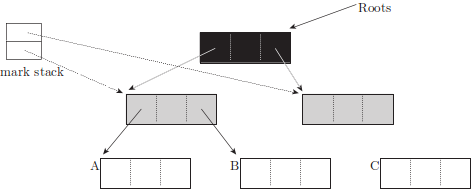
\includegraphics{figures/mrkswp_1}
  \caption[Σήμανση με τριχρωματική αφαίρεση]
    {Σήμανση με τριχρωματική αφαίρεση. Τα μαύρα αντικείμενα καθώς
     και τα παιδιά αυτών έχουν επεξεργασθεί από το συλλέκτη. Ο
     συλλέκτης γνωρίζει την ύπαρξη των γκρι αντικειμένων αλλά
     δεν έχει ολοκληρώσει την επεξεργασία τους. ο συλλέκτης δεν
     έχει επισκεφθεί ακόμη τα λευκά αντικείμενα (και μερικά δε
     τα επισκεφθεί ποτέ).}
  \label{fig:mrkswp_1}
\end{figure}

Ο αλγόριθμος της συλλογής με σήμανση και εκκαθάριση διατηρεί
μια σημαντική αναλλοίωτη: στο τέλος κάθε επανάληψης του
βρόχου σήμανσης δεν υπάρχουν αναφορές από μαύρα προς λευκά 
αντικείμενα. Επομένως κάθε λευκό προσβάσιμο αντικείμενο
είναι προσβάσιμο από κάποιο γκρι αντικείμενο. Η μη διατήρηση
της αναλλοίωτης διακινδυνεύει τη μη σήμανση ενός ζωντανού
απογόνου ενός μαύρου αντικειμένου (και κατ' επέκταση τη
λανθασμένη εκκαθάριση αυτού) καθώς ο συλλέκτης δεν 
επανεξετάζει μαύρα αντικείμενα. Η τριχρωματική αφαίρεση
είναι ιδιαίτερα χρήσιμη κατά τη θεώρηση αλγορίθμων για
ταυτόχρονη συλλογή σκουπιδιών, όπου τα νήματα τροποποιητές
εκτελούνται ταυτόχρονα με τα νήματα συλλέκτες.

\section{Σήμανση με χρήση bitmap}
Ένα bit σήμανσης συνήθως αποθηκεύεται στην επικεφαλίδα του
αντικειμένου. Εναλλακτικά, τα bits σήμανσης μπορούν να αποθηκεύονται
σε ένα ξεχωριστό bitmap στην άκρη του σωρού που συσχετίζει
κάθε ένα bit με κάθε πιθανή διεύθυνση στη μνήμη όπου μπορεί
να αποθηκευθεί ένα αντικείμενο. Ο απαιτούμενος χώρος για την
αποθήκευση του bitmap εξαρτάται από τις απαιτήσεις ευθυγράμμισης
της εικονικής μηχανής. Μπορεί να χρησιμοποιηθεί είτε ένα
καθολικό bitmap είτε αν ο σωρός είναι οργανωμένος σε μπλοκ
ένα bitmap ανά μπλοκ. Η τελευταία οργάνωση έχει ως πλεονέκτημα
πώς δεν σπαταλάται χώρος στην περίπτωση που ο σωρός δεν είναι
συνεχόμενος. Ο πίνακας bitmap για κάθε μπλοκ μπορεί να αποθηκευθεί
σε μία σταθερή θέση του μπλοκ, κάτι το οποίο ωστόσο διακινδυνεύει
την υποβάθμιση της επίδοσης, καθώς τα bitmap θα ανταγωνίζονται
για τα ίδια σύνολα σε μία συσχετιστική κρυφή μνήμη. Επιπλέον,
η πρόσβαση στο bitmap αυτόματα σημαίνει το άγγιγμα της αντίστοιχης
σελίδας. Για να αντιμετωπισθεί το πρώτο πρόβλημα, η θέση ενός
bitmap στο μπλοκ μπορεί να μεταβάλλεται και να προκύπτει για
παράδειγμα ως αποτέλεσμα της εφαρμογής μιας συνάρτησης κατακερματισμού
στη διεύθυνση του μπλοκ. Εναλλακτικά, το bitmap μπορεί να αποθηκευθεί
εκτός του μπλοκ, χρησιμοποιώντας όμως έναν πίνακα που δεικτοδοτείται
από μπλοκ (με πιθανή και πάλι χρήση κάποιας συνάρτησης κατακερματισμού).
Η τεχνική αυτή αντιμετωπίζει και τα δύο προβλήματα ταυτόχρονα.

Οι πίνακες bitmap αρκούν στην περίπτωση που η συλλογή απασχολεί
μόνο ένα νήμα σήμανσης. Διαφορετικά, η ενημέρωση ενός bit σε
έναν πίνακα bitmap είναι ευάλωτη στην απώλεια ενημερώσεων ενώ
αντίθετα η ενημέρωση ενός bit στην επικεφαλίδα ενός αντικειμένου
κινδυνεύει απλώς την εγγραφή της ίδιας τιμής εις διπλούν. Πολλοί
συλλέκτες χρησιμοποιούν πίνακες bytemap για να καταστήσουν τις
καταστάσεις συναγωνισμού ακίνδυνες. Εναλλακτικά, η τροποποίηση
ενός bit σε έναν πίνακα bitmap πρέπει να γίνεται με τη χρήση
συγχρονισμένων λειτουργιών. Στην πράξη η κατάσταση είναι επίσης
περίπλοκη όσον αφορά μεμονωμένα bits της επικεφαλίδας σε συστήματα
που επιτρέπουν ταυτόχρονη εκτέλεση συλλέκτη και τροποποιητή, καθώς
οι λέξεις της επικεφαλίδας φιλοξενούν μεταξύ άλλων και δεδομένα
τα οποία μπορεί να προσπελάσει ο τροποποιητής, όπως κλειδώματα
και κωδικοί κατακερματισμού (hash codes). Μια προσεκτική σχεδίαση
μπορεί να τοποθετήσει τα παραπάνω δεδομένα σε διαφορετικές
λέξεις της επικεφαλίδας και να εξαλείψει την ανάγκη για ατομική
τροποποίηση των bits σήμανσης αυτής.

Η χρήση bitmap σήμανσης παρουσιάζει έναν αριθμό από πλεονεκτήματα.
Ένα bitmap αποθηκεύει τα bit σήμανσης πιο πυκνά σε σύγκριση με
την αποθήκευσή τους στις επικεφαλίδες των αντικειμένων. Η χρήση
bitmap σήμανσης κατά τη συλλογή με σήμανση και εκκαθάριση συνεπάγεται
πώς η φάση της σήμανσης δεν τροποποιεί κανένα αντικείμενο, παρά
διαβάζει τα πεδία δείκτες των ζωντανών αντικειμένων. Με εξαίρεση
τη φόρτωση του πεδίου περιγραφητή τύπου, κανένα άλλο τμήμα αντικειμένων
που δεν περιέχουν δείκτες δεν προσπελαύνεται. Η φάση της εκκαθάρισης
δε θα διαβάσει από ούτε και θα γράψει σε κάποιο ζωντανό αντικείμενο,
παρότι μπορεί να ενημερώσει πεδία αντικειμένων σκουπιδιών στα 
πλαίσια της ανάκτησης της μνήμης που αυτά καταλαμβάνουν (για παράδειγμα
για να εισάγει ένα αντικείμενο σε μια ελεύθερη λίστα). Συνεπώς 
η σήμανση με χρήση bitmap έχει την τάση να τροποποιεί λιγότερες 
λέξεις μνήμης, με αποτέλεσμα ο αριθμός των βρώμικων μπλοκ κρυφής
μνήμης που πρέπει να αντιγραφούν στην κύρια μνήμη να μειώνεται.

Η σήμανση με τη χρήση bitmap υιοθετήθηκε αρχικά για ένα συντηρητικό
συλλέκτη που σχεδίασαν οι Boehm και Wieser \cite{DBLP:journals/spe/BoehmW88}
για την παροχή αυτόματης διαχείρισης μνήμης σε υλοποιήσεις μη 
συνεργατικών γλωσσών όπως η C και η C++. Σε συστήματα με ακριβή
πληροφορία τύπων η ταυτοποίηση κάθε θέσης μνήμης που περιέχει
ένα δείκτη είναι ακριβής ανεξάρτητα από το αν αυτή αφορά το 
εσωτερικό κάποιου αντικειμένου, τη στοίβα ή κάποια καθολική μεταβλητή.
Οι \textbf{συντηρητικοί (conservative)} συλλέκτες αντίθετα δεν
λαμβάνουν αυτό το επίπεδο υποστήριξης από το μεταγλωττιστή ή 
το σύστημα εκτέλεσης και για αυτό προβαίνουν σε συντηρητικές
αποφάσεις όσον αφορά την ταυτοποίηση δεικτών. Εάν η τιμή που
βρίσκεται σε μια θέση μνήμης μοιάζει αρκετά με δείκτη, ο συλλέκτης
αποφασίζει πώς πράγματι είναι. Είναι εμφανές πώς η συντηρητική
συλλογή σκουπιδιών ενδέχεται εσφαλμένα να διερμηνεύσει μια θέση
μνήμης ως δείκτη, κάτι που έχει δύο συνέπειες όσον αφορά την 
ασφάλεια. Πρώτον, ο συλλέκτης δεν επιτρέπεται να μεταβάλλει το
περιεχόμενο καμίας θέσης μνήμης στο χώρο διευθύνσεων του τροποποιητή
(συμπεριλαμβανομένων των ριζών). Αυτό αποκλείει αμέσως αλγορίθμους
που μετακινούν αντικείμενα, καθώς αυτό θα απαιτούσε την ενημέρωση
κάθε αναφοράς προς ένα μετακινηθέν αντικείμενο. Επίσης αποκλείει
την αποθήκευση των bits σήμανσης στις επικεφαλίδες των αντικειμένων
καθώς ένα 'αντικείμενο' για το οποίο γίνεται λόγος μπορεί να μην
είναι αντικείμενο αν η πρόσβαση σε αυτό έγινε από την εσφαλμένη
θεώρηση μιας τιμής ως δείκτη. Η τροποποίηση της τιμής ενός bit
μπορεί να καταστρέψει τα δεδομένα του χρήστη. Δεύτερον, η ελαχιστοποίηση
της πιθανότητας ο τροποποιητής να προσπελαύνει δεδομένα του
συλλέκτη είναι πολύ χρήσιμη. Η προσθήκη μιας επικεφαλίδας στην
αρχή ενός αντικειμένου είναι πιο ριψοκίνδυνη από την αποθήκευση
των μεταδεδομένων του συλλέκτη όπως τα bits  σήμανσης σε μία
ξεχωριστή δομή δεδομένων.

Σύμφωνα με τον Boehm \cite{DBLP:conf/iwmm/Boehm00}, ένα επιπλέον
κίνητρο για τη σήμανση με χρήση bitmap είναι η ανάγκη για ελαχιστοποίηση 
της σελιδοποίησης που προκαλείται από τη δράση του συλλέκτη.
Στα σύγχρονα συστήματα πάντως η πρόκληση της παραμικρής σελιδοποίησης
από το συλλέκτη θεωρείται απαράδεκτη. Το ερώτημα είναι κατά πόσο
η σήμανση με χρήση bitmap μπορεί να βελτιώσει την επίδοση της
κρυφής μνήμης. Σύμφωνα με τους Hayes \cite{DBLP:conf/oopsla/Hayes91}
και Jones και Ryder \cite{DBLP:conf/iwmm/JonesR08} τα αντικείμενα
έχουν μια τάση να ζουν και να πεθαίνουν σε συστάδες. Πολλοί εκχωρητές 
προσπαθούν να τοποθετήσουν τα αντικείμενα σε γειτονικές θέσεις
μνήμης. Η εκκαθάριση με χρήση bitmap παρουσιάζει δύο πλεονεκτήματα.
Πρώτον, επιτρέπει το μαζικό έλεγχο των bits/bytes σήμανσης για 
τα αντικείμενα μιας συστάδας, καθώς είτε όλα θα έχουν τη λογική
τιμή 0 είτε όλα θα έχουν τη λογική τιμή 1. Άμεση συνέπεια του
γεγονότος αυτού είναι πώς είναι εύκολο να προσδιορισθεί από το
bitmap το κάτα πόσο ένα μπλοκ μνήμης αποτελείται μόνο από
σκουπίδια και άρα μπορεί να επιστραφεί ολόκληρο στον εκχωρητή.

Ο Garner κ.ά \cite{DBLP:conf/iwmm/GarnerBF07} χρησιμοποιούν μια
υβριδική προσέγγιση, συσχετίζοντας κάθε μπλοκ των ξεχωριστών 
ελεύθερων λιστών από μπλοκ διαφορετικού μεγέθους με ένα byte
και ταυτόχρονα αποθηκεύοντας ένα bit στην επικεφαλίδα κάθε
αντικειμένου. Το byte έχει την τιμή 0xFF αν και μόνο αν το
αντίστοιχο μπλοκ έχει ένα τουλάχιστον ζωντανό αντικείμενο.
Με τον τρόπο αυτό το byte-map επιτρέπει στον εκκαθαριστή να
εντοπίζει εύκολα τα μπλοκ που δεν έχουν κανένα ζωντανό αντικείμενο
και στη συνέχεια να τα ανακυκλώνει ολόκληρα. Το βασικό πλεονέκτημα
της προσέγγισης αυτής είναι πώς τόσο το bit στην επικεφαλίδα ενός 
αντικειμένου όσο και το αντίστοιχο byte του byte-map που αφορά
το μπλοκ στο οποίο αυτό ζει μπορούν να εγγράφονται χωρίς τη
χρήση συγχρονισμένων λειτουργιών.

\begin{algorithm}[H]
  \caption{Σήμανση με bitmap (Printezis \& Detlefs)}
  \label{alg:ms_4}
  \begin{algorithmic}[1]
    \Procedure{mark}{\null}
      \State $cur \gets$ \Call{nextInBitmap}{\null}
      \While{$cur < HeapEnd$}
        \State \Call{add}{$worklist$, $cur$}
        \State \Call{markStep}{$cur$}
        \State $cur \gets$ \Call{nextInBitmap}{\null}
      \EndWhile
    \EndProcedure
    \Statex
    \Procedure{markStep}{$start$}
      \While{\textbf{not} \Call{isEmpty}{$worklist$}}
        \State $ref \gets$ \Call{remove}{$worklist$}
        \ForAll{$fld \in Pointers(ref)$}
          \State $child \gets *fld$
          \If{$child \neq \textbf{null}$ \textbf{and} \textbf{not} \Call{isMarked}{$child$}}
            \State $\Call{setMarked}{child}$
            \If{$child < start$}
              \State \Call{add}{$worklist$, $child$}
            \EndIf
          \EndIf
        \EndFor
      \EndWhile
    \EndProcedure
  \end{algorithmic}
\end{algorithm}

Οι Printezis και Detlefs \cite{DBLP:conf/iwmm/PrintezisD00}
χρησιμοποιούν bitmap για να μειώσουν τον απαιτούμενο χώρο
για τις στοίβες σήμανσης σε έναν σχεδόν-ταυτόχρονο, γενεαλογικό
συλλέκτη. Αρχικά, ως συνήθως οι ρίζες του τροποποιητή σημαίνονται
με την εγγραφή της λογικής τιμής ορισμένων bits στο bitmap.
Στη συνέχεια, το νήμα σήμανσης σαρώνει γραμμικά το bitmap αναζητώντας
για ζωντανά αντικείμενα. Ο αλγόριθμος \ref{alg:bitmap-marking}
διατηρεί την ακόλουθη αναλλοίωτη: τα σημασμένα αντικείμενα
που βρίσκονται σε χαμηλότερες διευθύνσεις από την τιμή του
δείκτη $cur$ στη διαδικασία \textproc{mark} είναι μαύρα,
ενώ τα αντικείμενα που βρίσκονται σε υψηλότερες διευθύνσεις
είναι γκρι. Όταν εντοπίζεται το επόμενο ζωντανό (σημασμένο)
αντικείμενο, αυτό ωθείται στη στοίβα και ο έλεγχος περνά
στη διαδικασία \textproc{markStep}. Η τελευταία εκτελεί έναν
βρόχο while προκειμένου να αποκαταστήσει την αναλλοίωτη:
αντικείμενα εξωθούνται από τη στοίβα και τα παιδιά τους
σημαίνονται αναδρομικά μέχρις ότου αυτή εκκενωθεί. Αν ένα
αντικείμενο βρίσκεται σε χαμηλότερη διεύθυνση μνήμης από
την τρέχουσα τιμή του δείκτη $cur$, αυτό εισάγεται στη στοίβα
σήμανσης, αλλιώς η επεξεργασία του αναβάλλεται για αργότερα. 
Η βασική διαφορά αυτού του αλγορίθμου και του αλγορίθμου 
\ref{alg:marking} είναι αφορά στην εισαγωγή των παιδιών ενός 
αντικειμένου στη στοίβα σήμανσης. Τα αντικείμενα σημαίνονται 
αναδρομικά μόνο αν αυτά βρίσκονται πίσω από το μαύρο μέτωπο κύματος 
που κινείται γραμμικά στο σωρό. Παρότι η πολυπλοκότητα του αλγορίθμου 
αυτού είναι γραμμική ως προς το μέγεθος του χώρου που συλλέγεται, 
στην πράξη η αναζήτηση σε ένα bitmap είναι φθηνή.
 
\section{Οκνηρή εκκαθάριση}
Η χρονική πολυπλοκότητα της σήμανσης είναι $O(L)$, όπου $L$ το 
συνολικό μέγεθος των ζωντανών αντικειμένων του σωρού, ενώ η 
χρονική πολυπλοκότητα της εκκαθάρισης $O(H)$, όπου $H$ το μέγεθος 
του σωρού. Καθώς $H>L$, εκ πρώτης όψεως φαίνεται πώς το κόστος 
της εκκαθάρισης κυριαρχεί στο κόστος του αλγορίθμου συλλογής με 
σήμανση και εκκαθάριση, κάτι που στην πράξη δεν παρατηρείται. To 
``κυνήγι'' δεικτών στη φάση της σήμανσης οδηγεί σε τελείως μη 
προβέψιμα μοτίβα πρόσβασης στη μνήμη, ενώ αντίθετα η συμπεριφορά 
της εκκαθάρισης είναι πολύ πιο προβλέψιμη. Επιπροσθέτως, το 
κόστος της εκκαθάρισης ενός αντικειμένου είναι πολύ μικρότερο από 
το κόστος της εξερεύνησης του υπογράφου των αντικειμένων με ρίζα 
αυτό. Η προφόρτωση (prefetching) αντικειμένων αποτελεί έναν τρόπο 
βελτίωσης της συμπεριφοράς της εκκαθάρισης όσον αφορά τη μνήμη 
cache. Για να αποφύγουν τον κατακερματισμό της μνήμης οι εκχωρητές 
πολλών διαχειριστών μνήμης που υποστηρίζουν συλλέκτες με σήμανση 
και εκκαθάριση τοποθετούν αντικείμενα του ίδιου μεγέθους σε 
συνεχόμενες διευθύνσεις μνήμης, οδηγώντας με τον τρόπο αυτό σε
σταθερό βήμα μοτίβου πρόσβασης μνήμης κατά την εκκαθάριση μπλοκ
από αντικείμενα του ίδιου μεγέθους. Αυτή η προσέγγιση δεν 
επιτρέπει μόνο προφόρτωση λογισμικού αλλά είναι ιδανική και για
τους μηχανισμούς προφόρτωσης υλικού που διαθέτουν οι σύγχρονοι
επεξεργαστές.

Μπορούν οι χρόνοι πάυσης των νημάτων τροποποιητών για την εκτέλεση 
της φάσης της εκκαθάρισης να ελαττωθούν ή και να εξαλειφθούν 
πλήρως; Παρατηρούμε δύο ιδιότητες των αντικειμένων και των bit
σήμανσης αυτών. Πρώτον, από τη στιγμή που ένα αντικείμενο γίνεται
σκουπίδι, παραμένει σκουπίδι: δεν μπορεί να προσπελασθεί ή να
αναστηθεί από κάποιο νήμα τροποποιητή. Δεύτερον, τα νήματα
τροποποιητές δεν έχουν πρόσβαση στα bit σήμανσης. Επομένως η
εκκαθάριση μπορεί να ανατεθεί σε ξεχωριστά νήματα, τα οποία 
εκτελούνται ταυτόχρονα με τα νήματα τροποποιητές. Μια απλούστερη
λύση είναι η \textbf{οκνηρή εκκαθάριση}, HUGHES.
Η τεχνική ουσιαστικά πληρώνει το κόστος της εκκαθάρισης σε δόσεις 
με την εκκαθάριση να πραγματοποιείται από τον εκχωρητή. Στην 
απλούστερη εκδοχή η συνάρτηση \textproc{allocate} αυξάνει τον
δείκτη εκκαθάρισης μέχρις ότου βρει επαρκή χώρο σε μια ακολουθία
μη σημασμένων αντικειμένων. Ωστόσο, η εκκαθάριση ενός μπλοκ κάθε 
φορά με πολλά αντικείμενα είναι πιο αποδοτική. 

Ο αλγόριθμος \ref{alg:mrkswp5} επενεργεί σε ένα μπλοκ κάθε 
φορά. Είναι σύνηθες οι εκχωρητές να τοποθετούν στο ίδιο μπλοκ
ισομεγέθη αντικείμενα. Κάθε κλάση μεγέθους έχει ένα ή και 
περισσότερα μπλοκ εκχώρησης μνήμης καθώς και μία λίστα ανάκτησης
($reclaimList$) από μπλοκ που δεν έχουν ακόμη εκκαθαρισθεί.
Ως συνήθως ο συλλέκτης σημαίνει όλα τα ζωντανά αντικείμενα στο 
σωρό αλλά αντί να εκκαθαρίσει πρόθυμα ολόκληρο το σωρό, αυτός
επιστρέφει τα τελείως άδεια από ζωντανά αντικείμενα μπλοκ στον
εκχωρητή. Τα υπόλοιπα μπλοκ προστίθενται στην κατάλληλη λίστα
ανάκτησης με βάση το μέγεθος των αντικειμένων που φιλοξενούν.
Με τη λήξη της φάσης διακοπής του κόσμου τα νήματα τροποποιητές
επανεκκινούνται. Η συνάρτηση \textproc{allocate} αρχικά επιχειρεί
την απόκτηση μιας ελεύθερης θέσης από την αντίστοιχη κλάση 
μεγέθους. Αν η προσπάθεια αποτύχει, καλείται ο οκνηρός εκκαθαριστής
ο οποίος εκκαθαρίζει ένα ή περισσότερα εναπομείναντα μπλοκ της
αντίστοιχης λίστας $reclaimList$ μέχρις ότου το αίτημα μπορεί
να ικανοποιηθεί. Τι συμβαίνει στην περίπτωση όπου η λίστα των
όχι ακόμη εκκαθαρισμένων μπλοκ είναι κενή ή δεν υπάρχει ελεύθερη
θέση σε κανένα από τα εκκαθαρισμένα μπλοκ; Η απάντηση είναι πώς
ο εκκαθαριστής προσπαθεί να αποκτήσει ένα ολόκληρο ελεύθερο μπλοκ
από έναν κατώτερου επιπέδου εκχωρητή μπλοκ. Το φρέσκο μπλοκ
στη συνέχεια αρχικοποιείται με ρύθμιση των μεταδεδομένων αυτού
(όπως για παράδειγμα με τη δημιουργία ενός πίνακα με byte σήμανσης).
Αν πάλι δεν υπάρχουν διαθέσιμα φρέσκα μπλοκ, απαιτείται η κλήση
του συλλέκτη.

Υπάρχει ένα λεπτό ζήτημα όσον αφορά την οκνηρή εκκαθάριση σε
έναν οργανωμένο κατά μπλοκ σωρό. Ο Hughes [1982] δουλεύει με 
έναν συνεχόμενο σωρό και επομένως εξασφαλίζει πώς ο εκχωρητής θα
εκκαθαρίσει κάθε αντικείμενο πριν ξεμείνει από χώρο και καλέσει
το συλλέκτη. Ωστόσο, η οκνηρή εκκαθάριση ξεχωριστών κλάσεων
ως προς το μέγεθος δεν μπορεί να το εξασφαλίσει καθώς είναι σχεδόν
σίγουρο πώς ο εκκαθαριστής θα εξαντλήσει μια κλάση μεγέθους (και
όλα τα άδεια μπλοκ αυτής) πριν προχωρήσει στην εκκαθάριση μπλοκ
που ανήκουν σε διαφορετικές κλάσεις μεγέθους. Το γεγονός αυτό
οδηγεί σε δύο προβλήματα. Πρώτον, αντικείμενα σκουπίδια σε μη
εκκαθαρισμένα μπλοκ δεν αποδεσμεύονται, οδηγώντας σε διαρροή 
μνήμης. Αν το μπλοκ περιλαμβάνει ένα ζωντανό αντικείμενο, η 
παραπάνω διαρροή είναι αβλαβής καθώς τα αντικείμενα του μπλοκ 
δε θα ανακυκλωθούν ούτως ή άλλως πριν ο συλλέκτης πραγματοποιήσει
ένα αίτημα για αντικείμενο της κλάσης μεγέθους στην οποία ανήκει
το μπλοκ. Δεύτερον, αν όλα τα αντικείμενα σε ένα μπλοκ διαδοχικά
μετατραπούν σε σκουπίδια, έχει χαθεί η δυνατότητα ανάκτησης όλου
του μπλοκ μονομιάς.

Η απλούστερη λύση είναι η ολοκλήρωση της εκκαθάρισης όλων των
μπλοκ του σωρού πριν την έναρξη της σήμανσης. Ωστόσο, μπορεί
να είναι προτιμότερο να δοθούν σε ένα μπλοκ περισσότερες ευκαιρίες
οκνηρής εκκαθάρισής του. Ο Garner κ.ά \cite{DBLP:conf/iwmm/GarnerBF07}
πληρώνουν ένα μικρό ποσό διαρροής για να αποφύγουν το κόστος
της πρόθυμης εκκαθάρισης στο σύστημα Jikes RVM/MMTk των Blackburn
κ.ά \cite{DBLP:conf/iwmm/BlackburnH04}. Πιο συγκεκριμένα, αντί
ενός bit, χρησιμοποιούν ένα φραγμένο ακέραιο για τη σήμανση των
αντικειμένων. Αυτό συνήθως δεν επιφέρει επιπλέον κόστος σε χώρο
καθώς υπάρχει χώρος παραπάνω από ένα bit αν οι σημάνσεις αποθηκεύονται
στις επικεφαλίδες των αντικειμένων και συχνά ξεχωριστές δομές
σήμανσης χρησιμοποιούν byte αντί για bit. Κάθε κύκλος συλλογής
αυξάνει την τιμή σήμανσης κατά $2^K$, όπου $K$ το μέγεθος της
λέξης σήμανσης σε bits, με την τιμή σήμανσης να επανέρχεται
προφανώς στο $0$ σε περίπτωση υπερχείλισης. Με τον τρόπο αυτό,
ο συλλέκτης μπορεί να ξεχωρίσει ένα αντικείμενο που έχει σημανθεί
στον τρέχοντα κύκλο συλλογής από ένα αντικείμενο που είχε
σημανθεί σε κάποιον προηγούμενο κύκλο συλλογής. Μόνο τα αντικείμενα
με την τρέχουσα τιμή σήμανσης θεωρούνται σημασμένα. Η μηδενική
τιμή σήμανσης είναι ασφαλής καθώς, ακριβώς πριν την εμφάνισή
της, κάθε ζωντανό αντικείμενο στο σωρό είναι είτε μη σημασμένο
(η μνήμη του εκχωρήθηκε μετά τον προηγούμενο κύκλο συλλογής),
είτε έχει τη μέγιστη τιμή σήμανσης. Κάθε αντικείμενο που είναι
σημασμένο με την επόμενη τιμή σήμανσης πρέπει να έχει σημανθεί
κάποιο πολλαπλάσιο του $2^K$ αριθμό συλλογών πριν: επομένως
είναι αιωρούμενο σκουπίδι και δε σημαίνεται από το νήμα σήμανσης.
Η πιθανή προκύπτουσα διαρροή αντιμετωπίζεται σε ένα βαθμό
με τη σήμανση ολόκληρων μπλοκ. Οποτεδήποτε ο MMTk συλλέκτης
σημαίνει ένα αντικείμενο, σημαίνει επίσης και το αντίστοιχο
μπλοκ. Αν κάνενα από τα αντικείμενα ενός μπλοκ δεν είναι
σημασμένο με την τρέχουσα τιμή σήμανσης, τότε ούτε και το
μπλοκ είναι και συνεπώς μπορεί να ανακτηθεί ολόκληρο, όπως
στον αλγόριθμο~\ref{alg:mrkswp5}. Λαμβάνοντας υπόψη την τάση
των αντικειμένων να ζουν και να πεθαίνουν σε συστάδες,
αναμένει κανείς πώς η παραπάνω τεχνική είναι αποδοτική.

Η οκνηρή εκκαθάριση προσφέρει έναν αριθμό από πλεονεκτήματα.
Αρχικά έχει καλή τοπικότητα: μία θέση μνήμης ενός πρώην σκουπιδιού 
τείνει να χρησιμοποιηθεί σύντομα μετά την εκκαθάριση του τελευταίου.
Επιπλέον, η αλγοριθμική πολυπλοκότητα της συλλογής με σήμανση και
εκκαθάριση είναι πλέον γραμμική ως προς το μέγεθος των ζωντανών
αντικειμένων του σωρού, ίδια με την πολυπλοκότητα της συλλογής με
αντιγραφή που εξετάζουμε στο κεφάλαιο \ref{ch:copy}. Συγκεκριμένα,
ο Boehm \cite{boehm1995dynamic} επισημαίνει πώς η συλλογή με σήμανση και οκνηρή
εκκαθάριση παρουσιάζει βέλτιστες επιδόσεις στις ίδιες συνθήκες με
τη συλλογή με αντιγραφή: όταν το μεγαλύτερο μέρος του σωρού είναι
άδειο, καθώς η αναζήτηση μη σημασμένων αντικειμένων από την οκνηρή
εκκαθάριση θα ολοκληρωθεί γρήγορα.

\begin{algorithm}
  \caption{Οκνηρή εκκαθάριση σε οργανωμένο κατά μπλοκ σωρό}
  \label{alg:mrkswp5}
  \begin{algorithmic}[1]
    \Procedure{collect}{\null}
      \State \textbf{atomic}
      \State \Call{markFromRoots}{\null}
      \ForAll{$block \; \textbf{in} \; blocks$}
        \If{\textbf{not} \Call{isMarked}{$block$}} \Comment{no objects marked in this block?}
          \State \Call{add}{$blockAllocator$, $block$} \Comment{return block to block allocator}
        \Else
          \State \Call{add}{$reclaimList$, $block$}
        \EndIf
      \EndFor
    \EndProcedure
    \Statex
    \Function{allocate}{$sz$}
      \State \textbf{atomic}
      \State $result \gets$ \Call{remove}{$sz$} \Comment{allocate from size class for sz}
      \If{$result = \textbf{null}$} \Comment{if no free slots for this size...}
        \State \Call{lazySweep}{$sz$} \Comment{sweep a little}
        \State $result \gets$ \Call{remove}{$sz$}
      \EndIf
      \State \Return{$result$} \Comment{if still null, collect}
    \EndFunction
    \Statex
    \Procedure{lazySweep}{$sz$}
      \Repeat
        \State $block \gets$ \Call{nextBlock}{$reclaimList$, $sz$}
        \If{$block \neq \textbf{null}$}
          \State \Call{sweep}{$start(block)$, $end(block)$}
          \If{\Call{spaceFound}{$block$}}
            \State \Return{\null}
          \EndIf
        \EndIf
      \Until{$block = \textbf{null}$} \Comment{reclaim list for this size class is empty}
      \State \Call{allowSlow}{$sz$}
    \EndProcedure
    \Statex
    \Procedure{allocSlow}{$sz$} \Comment{allocation slow path}
      \State $block \gets$ \Call{allocateBlock}{\null}
      \If{$block \neq \textbf{null}$} \Comment{from the block allocator}
        \State \Call{initialize}{$block$, $sz$}
      \EndIf
    \EndProcedure
  \end{algorithmic}
\end{algorithm}


\section{Ανακεφαλαίωση και θέματα προς εξέταση}
Παρά το γεγονός πώς είναι ο παλαιότερος αλγόριθμος συλλογής
σκουπιδιών, [McCarthy 1960] υπάρχουν διάφοροι λόγοι για τους 
οποίους η συλλογή με σήμανση και εκκαθάριση παραμένει ακόμα και
σήμερα ελκυστική επιλογή.

\subsection{Επιβάρυνση τροποποιητή}
Η απλούστερη εκδοχή του αλγορίθμου δεν επιβάλλει καμία επιβάρυνση
στις λειτουργίες \textproc{Read} και \textproc{Write} του 
τροποποιητή, σε αντίθεση για παράδειγμα με τη συλλογή με καταμέτρηση
αναφορών που εξετάζουμε στο κεφάλαιο \ref{ch:refcnt}.
Ωστόσο η συλλογή με σήμανση και εκκαθάριση συχνά χρησιμοποιείται
ως βασικός αλγόριθμος σε πιο εξεζητημένους συλλέκτες που απαιτούν
κάποιας μορφής συγχρονισμό μεταξύ συλλέκτη και τροποποιητή. Τόσο
οι γενεαλογικοί συλλέκτες (κεφάλαιο \ref{ch:gen}) όσο και
οι ταυτόχρονοι και αυξητικοί συλλέκτες (κεφάλαιο \ref{ch:conc})
απαιτούν από τον τροποποιητή να ενημερώνει το συλλέκτη οποτεδήποτε
τροποποιεί δείκτες.

\subsection{Ρυθμαπόδοση}
Σε συνδυασμό με την οκνηρή εκκαθάριση, η συλλογή με σήμανση και
εκκαθάριση προσφέρει υψηλή ρυθμαπόδοση. Η φάση της σήμανσης είναι
σχετικά φθηνή και κυριαρχείται από την καταδίωξη δεικτών. Χρειάζεται
απλώς να θέσει ένα bit/byte για κάθε ζωντανό αντικείμενο που
ανακαλύπτει, σε αντίθεση με τη συλλογή με αντιγραφή (κεφάλαιο
\ref{ch:copy}) ή με σήμανση και συμπύκνωση (κεφάλαιο \ref{ch:mrkcmp}) 
που αντιγράφουν ή μετακινούν αντικείμενα. Από την άλλη πλευρά, 
όπως και οι περισσότεροι συλλέκτες εξιχνίασης που εξετάζουμε
στα πρώτα κεφάλαια αυτής της εργασίας η συλλογή με σήμανση και
εκκαθάριση απαιτεί την διακοπή της εκτέλεσης των νημάτων τροποποιτών
κατά τη διάρκεια εκτέλεσης του συλλέκτη. Ο χρόνος παύσης ενός
κύκλου συλλογής εξαρτάται πρωτίστως από το πρόγραμμα που εκτελεί
ο τροποποιητής και την είσοδο αυτού και μπορεί εύκολα σε μερικές
περιπτώσεις να φθάσει και μερικά δευτερόλεπτα.

\subsection{Απαιτήσεις σε χώρο}
Η συλλογή με σήμανση και εκκαθάριση έχει σαφώς καλύτερη διαχείριση
χώρου από τη συλλογή με αντιγραφή. Ενδεχομένως να έχει καλύτερη
διαχείριση χώρου και από τη συλλογή με καταμέτρηση αναφορών. Τα
bits σήμανσης συχνά αποθηκεύονται χωρίς κόστος στις επικεφαλίδες
των αντικειμένων. Εναλλακτικά, αν χρησιμοποιείται ένας πίνακας
bitmap η επιβάρυνση σε χώρο εξαρτάται από τις απαιτήσεις ευθυγράμμισης
της αρχιτεκτονικής. Η συλλογή με καταμέτρηση αναφορών από την
άλλη πλευρά απαιτεί τη χρήση μίας λέξης μνήμης σε κάθε επικεφαλίδα
αντικειμένου για την αποθήκευση του μετρητή αναφορών του τελευταίου.
Η συλλογή με αντιγραφή έχει ακόμη χειρότερη διαχείριση του χώρου
αφού διαχωρίζει το σωρό σε δύο ισομεγέθεις ημιχώρους εκ των οποίων
μόνο ο ένας είναι ανά πάσα στιγμή διαθέσιμος στον τροποποιητή.
Από την άλλη πλευρά, οι συλλέκτες που δεν συμπυκνώνουν το σωρό,
όπως η συλλογή με σήμανση και εκκαθάριση αλλά και η συλλογή με
καταμέτρηση αναφορών απαιτούν από το διαχειριστή μνήμης τη χρήση
πιο περίπλοκων εκχωρητών. Οι επιπλέον δομές δεδομένων που απαιτούνται
για την υποστήρικη τέτοιων συλλεκτών προσθέτουν μια μη αμελητέα
επιβάρυνση. Επιπρόσθετα η συλλογή χωρίς συμπύκνωση συχνά συνοδεύεται
από κατακερματισμό της μνήμης.

Ο αλγόριθμος συλλογής σκουπιδιών με σήμανση και εκκαθάριση είναι
όπως εξηγήσαμε ένας αλγόριθμος εξιχνίασης. Ως τέτοιος, οφείλει 
να αναγνωρίσει πρώτα όλα τα ζωντανά αντικείμενα του σωρού πριν
ανακτήσει τη μνήμη που χρησιμοποείται από νεκρά αντικείμενα. 
Η διαδικασία αυτή είναι ακριβή και θα πρέπει να εκτελείται όσο 
πιο σπάνια γίνεται. Αυτό σημαίνει πώς πρέπει να αφιερωθεί ειδικός 
χώρος στο σωρό για τη λειτουργία των συλλεκτών εξιχνίασης. Αν 
τα ζωντανά αντικείμενα καταλαμβάνουν ένα μεγάλο μέρος του σωρού 
και οι εκχωρητές εκχωρούν πολύ συχνά μνήμη ο συλλέκτης με σήμανση 
και εκκαθάριση θα καλείται πολύ συχνά. O Jones [1996] επισημαίνει 
πώς για σωρούς μεσαίου και μεγάλου μεγέθους το ποσοστό του σωρού 
που αφιερώνεται στον ειδικό χώρο για τις λειτουργίες του συλλέκτη 
μπορεί να κυμαίνεται από 20\% έως και 50\%. Οι Hertz και Berger
[2005] \cite{DBLP:conf/oopsla/HertzB05} πάντως δείχνουν πώς
η αυτόματη διαχείριση μνήμης προγραμμάτων στη γλώσσα Java με
τη χρήση συλλογής με σήμανση και εκκαθάριση ενδέχεται να απαιτήσει
έναν σωρό ακόμη και μερικές φορές μεγαλύτερο σε μέγεθος προκειμένου
να πετύχει την ίδια ρυθμαπόδοση με την χειρωνακτική διαχείριση
μνήμης αυτών με ρητή αποδέσμευση.

\subsection{Μετακίνηση ή όχι;}
Η μη μετακίνηση αντικειμένων παρουσιάζει πλεονεκτήματα και
μειονεκτήματα. Το βασικό πλεονέκτημα που προκύπτει από τη μη
μετακίνηση αντικειμένων είναι πώς καθιστά τη συλλογή με σήμανση
και εκκαθάριση κατάλληλη για χρήση σε περιβάλλοντα όπου δεν 
υπάρχει συνεργασία μεταξύ μεταγλωττιστή της γλώσσας και συλλέκτη
σκουπιδιών. Χωρίς έγκυρη πληροφορία τύπων, οι ρίζες του τροποποιητή
και πεδία δείκτες αντικειμένων δεν γίνεται να ενημερωθούν με 
νέες διευθύνσεις μετακινηθέντων αντικειμένων. Αυτό συμβαίνει 
λόγω της έλλειψης βεβαιότητας σχετικά με το αν μια μεταβλητή 
ή ένα πεδίο στο εσωτερικό ενός αντικείμενου είναι δείκτης. 

Η ασφάλεια σε μη συνεργατικά συστήματα που διαχειρίζονται από
έναν συντηρητικό συλλέκτη αποτρέπει τον τελευταίο από την
τροποποίηση δεδομένων του χρήστη (συμπεριλαμβανομένων των
επικεφαλίδων αντικειμένων). Επιπλέον ενθαρρύνει την ξεχωριστή
αποθήκευση των μεταδεδομένων του συλλέκτη από τα μεταδεδομένα
του χρήστη και του συστήματος εκτέλεσης ώστε να μειωθεί η
πιθανότητα τροποποίησης των πρώτων από τον τροποποιητή. Για 
τους παραπάνω λόγους είναι επιθυμητή η αποθήκευση των bit/byte
σήμανσης σε πίνακες bitmap και όχι στις επικεφαλίδες των
αντικειμένων.

Το πρόβλημα με τη μετακίνηση αντικειμένων είναι πώς σε εφαρμογές
που τρέχουν για πολλή ώρα, ο σωρός τείνει να κατακερματίζεται.
Ο Robson \cite{DBLP:journals/jacm/Robson71, DBLP:journals/jacm/Robson74}
αποδεικνύει πώς οι εκχωρητές σε συστήματα διαχείρισης μνήμης που
χρησιμοποιούν μη μετακινούντα συλλέκτη απαιτούν $O(\log{\frac{max}{min}})$
περισσότερο χώρο από τον ελάχιστο δυνατό, όπου $min$ και $max$
το ελάχιστο και μέγιστο δυνατό μέγεθος αντικειμένων αντίστοιχα.
Συνεπώς ένας συλλέκτης δε συμπυκνώνει το σωρό με μεγάλη πιθανότητα
καλείται συχνότερα από έναν που το συμπυκνώνει. Ακόμη, όπως
σημειώθηκε πιο πάνω, ένα ποσοστό από 20\% έως και 50\% του σωρού
πρέπει να αφιερώνεται αποκλειστικά στη λειτουργία ενός συλλέκτη
εξιχνίασης ώστε να αποφευχθεί η αυξημένη συχνότητα κλήσης του
τελευταίου.

Για να ελαχιστοποιηθεί η μείωση της επίδοσης λόγω του κατακερματισμού,
πολλές εμπορικές υλοποιήσεις συλλεκτών οι οποίες διαχειρίζονται
μια περιοχή του σωρού με σήμανση και εκκαθάριση περιοδικά χρησιμοποιούν
και διαφορετικό αλγόριθμο όπως αυτόν με σήμανση και συμπύκνωση για
να εξαλείψουν τον κατακερματισμό. Συγκεκριμένα αυτό απαιτείται
αν η εφαρμογή δε διατηρεί σταθερό ρυθμό μεγεθών αντικειμένων ή
δεσμεύει μνήμη για πολλά μεγάλα αντικείμενα. Αν αρχίσει να δεσμεύει
μνήμη για μεγαλύτερα αντικείμενα από ότι πριν, ενδέχεται να προκύψουν
πολλές μικρές τρύπες στο σωρό που δε χρησιμοποιούνται πλέον για
τη δέσμευση μνήμης νέων αντικειμένων του ίδιου (μεγαλύτερου)
μεγέθους. Αντίστροφα, αν αρχίσει να δεσμεύει μνήμη για μικρότερα
αντικείμενα από ότι πριν, τα τελευταία μπορεί να φιλοξενούνται
σε κενά που προηγουμένως καταλαμβάνονταν από μεγαλύτερα αντικείμενα
οδηγώντας έτσι σε σπατάλη του αχρησιμοποίητου χώρου των κενών. 
Ο Dimpsey κ.ά \cite{DBLP:journals/ibmsj/DimpseyAK00}, όπως και
οι Blackburn και McKinley \cite{DBLP:conf/pldi/BlackburnM08}
ωστόσο παρατηρούν πώς η προσεκτική διαχείριση του σωρού μπορεί
να ελαττώσει την τάση για κατακερματισμό της μνήμης επωφελούμενη
την τάση των αντικειμένων να ζουν και να πεθαίνουν σε συστάδες.

\end{greek}
